\documentclass[12pt]{article}
\usepackage[margin=2.5cm]{geometry}
\usepackage{enumerate}
\usepackage{amsfonts}
\usepackage{amsmath}
\usepackage{fancyhdr}
\usepackage{amsmath}
\usepackage{amssymb}
\usepackage{amsthm}
\usepackage{mdframed}
\usepackage{graphicx}
\usepackage{subcaption}
\usepackage{adjustbox}
\usepackage{listings}
\usepackage{xcolor}
\usepackage{booktabs}
\usepackage[utf]{kotex}
\usepackage{hyperref}

\definecolor{codegreen}{rgb}{0,0.6,0}
\definecolor{codegray}{rgb}{0.5,0.5,0.5}
\definecolor{codepurple}{rgb}{0.58,0,0.82}
\definecolor{backcolour}{rgb}{0.95,0.95,0.92}

\lstdefinestyle{mystyle}{
    backgroundcolor=\color{backcolour},
    commentstyle=\color{codegreen},
    keywordstyle=\color{magenta},
    numberstyle=\tiny\color{codegray},
    stringstyle=\color{codepurple},
    basicstyle=\ttfamily\footnotesize,
    breakatwhitespace=false,
    breaklines=true,
    captionpos=b,
    keepspaces=true,
    numbers=left,
    numbersep=5pt,
    showspaces=false,
    showstringspaces=false,
    showtabs=false,
    tabsize=1
}

\lstset{style=mystyle}

\pagestyle{fancy}
\renewcommand{\headrulewidth}{0.4pt}
\lhead{Team Treehouse}
\rhead{Querying Relational Databases Part 4 Notes}

\begin{document}
\title{Querying Relational Databases Part 4 Notes}
\author{Team Treehouse}
\maketitle

\bigskip

\section{Join Queries}

\bigskip

\begin{itemize}
    \item Joins two or more tables into one
    \item Is used in tables with one to one relationship

    \begin{center}
    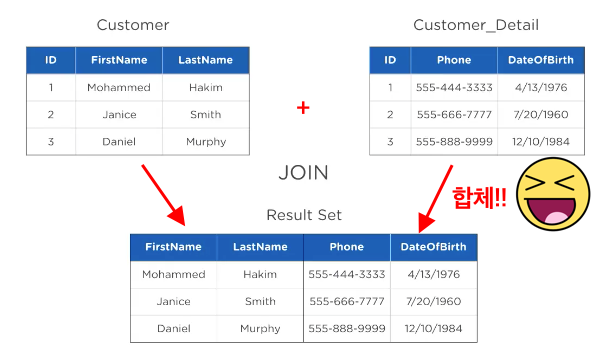
\includegraphics[width=0.8\linewidth]{images/part_4_notes_1.png}
    \end{center}
\end{itemize}

\bigskip

\section{Inner Joins}

\begin{center}
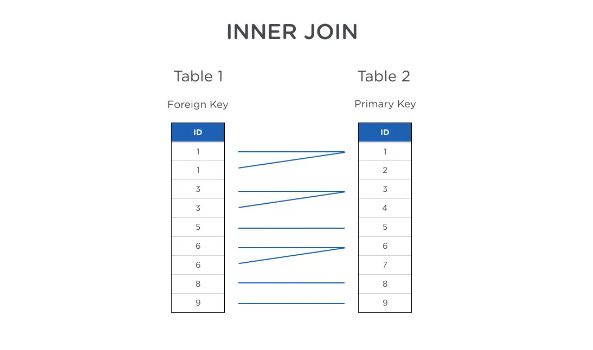
\includegraphics[width=\linewidth]{images/part_4_notes_3.png}
\end{center}

\bigskip

\begin{itemize}
    \item Is most common type of JOIN
    \item Is used for joining one to many relationships
    \item \textbf{Syntax:} SELECT \textit{columns name} FROM \textit{table 1 (many) name}
    INNER JOIN \textit{table 2 (one) name} ON \textit{table 1 name}.\textit{column name} = \textit{table 1 name}.\textit{column name};
    \begin{itemize}
        \item Can join more than 2 tables
    \end{itemize}

    \bigskip

    \underline{\textbf{Example:}}

    \bigskip

    \begin{lstlisting}[language=SQL]
    SELECT mk.MakeName = md.ModelName FROM make AS mk
    INNER JOIN model AS md ON mk.MakeId = md.MakeId;
    \end{lstlisting}

    \bigskip

    \begin{center}
    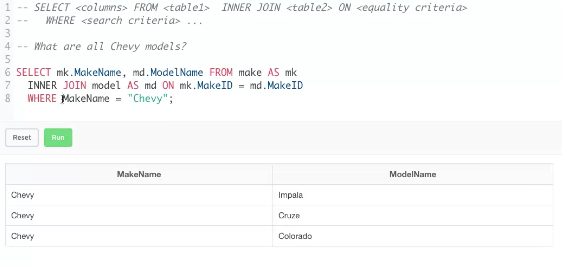
\includegraphics[width=0.8\linewidth]{images/part_4_notes_2.png}
    \end{center}

    \item In venn diagram, looks something like this

    \begin{center}
    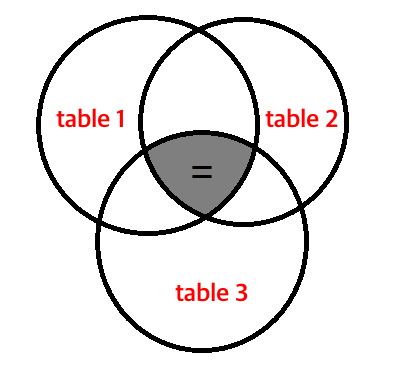
\includegraphics[width=0.4\linewidth]{images/part_4_notes_4.png}
    \end{center}
\end{itemize}

\bigskip

\section{Outer Join}

\bigskip

\begin{itemize}
    \item Is less common than inner join, but highly useful
    \item There are three types
    \begin{itemize}
        \item Left Outer Join
        \begin{center}
        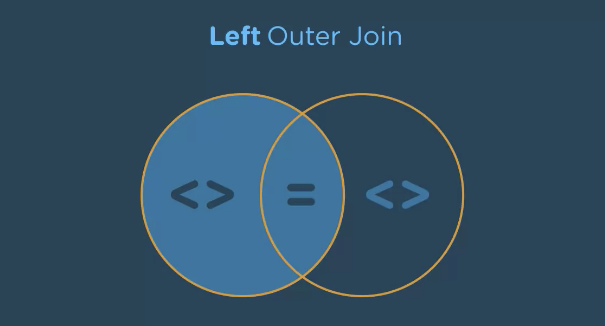
\includegraphics[width=0.6\linewidth]{images/part_4_notes_5.png}
        \end{center}

        \begin{itemize}
            \item \textbf{Syntax:} SELECT \textit{columns name} FROM \textit{table 1 name}
            LEFT OUTER JOIN \textit{table name 2} ON \textit{table 1 name}.\textit{column name} = \textit{table 1 name}.\textit{column name};
            \item joins tables with all columns from table 1 returned
        \end{itemize}

        \bigskip

        \item Right Outer Join

        \begin{center}
        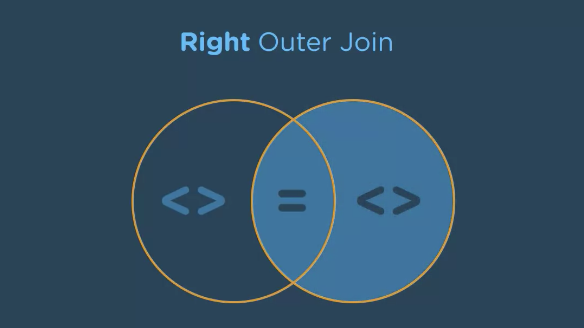
\includegraphics[width=0.6\linewidth]{images/part_4_notes_6.png}
        \end{center}

        \begin{itemize}
            \item \textbf{Syntax:} SELECT \textit{columns name} FROM \textit{table 1 name}
            RIGHT OUTER JOIN \textit{table name 2} ON \textit{table 1 name}.\textit{column name} = \textit{table 1 name}.\textit{column name};
            \item joins tables with all columns from table 2 returned
        \end{itemize}

        \item Full Outer Join
        \begin{center}
        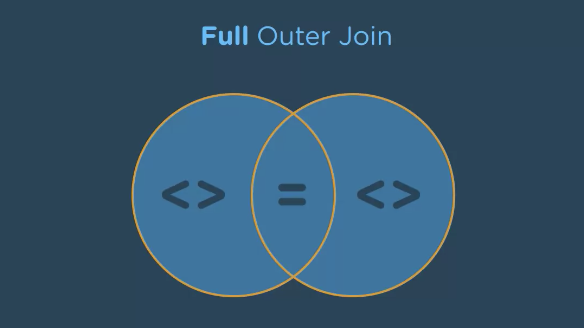
\includegraphics[width=0.6\linewidth]{images/part_4_notes_7.png}
        \end{center}

        \begin{itemize}
            \item \textbf{Syntax:} SELECT \textit{columns name} FROM \textit{table 1 name}
            FULL OUTER JOIN \textit{table name 2} ON \textit{table 1 name}.\textit{column name} = \textit{table 1 name}.\textit{column name};
            \item joins tables with all columns from both tables returned
        \end{itemize}

        \bigskip

        \underline{\textbf{Example:}}

        \bigskip

    \begin{lstlisting}[language=SQL]
    SELECT mk.MakeName, md.ModelName FROM make AS mk
    LEFT OUTER JOIN model AS md ON mk.MakeId = md.MakeId;
    \end{lstlisting}

        \bigskip

        \begin{center}
        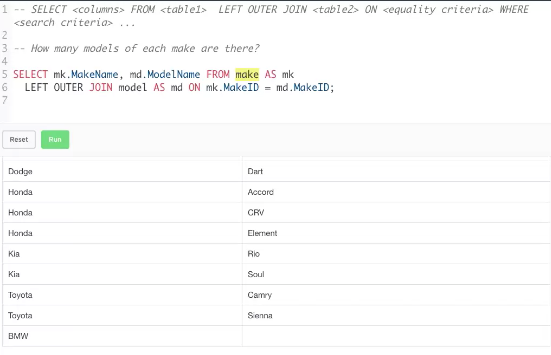
\includegraphics[width=\linewidth]{images/part_4_notes_8.png}
        \end{center}


    \end{itemize}
\end{itemize}

\bigskip

\section{Quiz 1}

\bigskip

\begin{enumerate}[1.]
    \item

    \begin{center}
    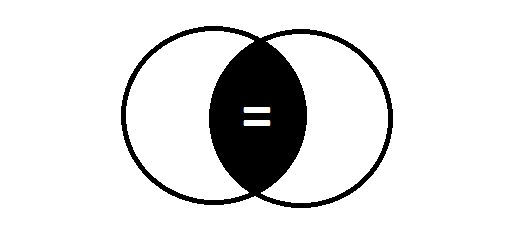
\includegraphics[width=\linewidth]{images/part_4_notes_9.png}
    \end{center}

    \bigskip

    This Venn Diagram represents what kind of JOIN:

    \begin{enumerate}[A.]
        \item INNER JOIN
        \item FULL JOIN
        \item RIGHT OUTER JOIN
        \item LEFT OUTER JOIN
    \end{enumerate}

    \bigskip

    \textbf{Answer:} A

    \item

    What is a JOIN?

    \bigskip

    \begin{enumerate}[A.]
        \item It is how a SQL query combines data from two tables into one result set.
        \item It is how a SQL query updates data in a table.
        \item It is how an application connects to a database.
        \item It is how one database connects to another database.
    \end{enumerate}

    \bigskip

    \textbf{Answer:} A

    \item

    Which is the most common type of JOIN?

    \bigskip

    \begin{enumerate}[A.]
        \item PIVOT JOIN
        \item OUTER JOIN
        \item TABULAR JOIN
        \item INNER JOIN
    \end{enumerate}

    \bigskip

    \textbf{Answer:} D

    \item

    A left outer join returns all data from the first -- or left -- table and
    only the data with matches in the second table.

    \bigskip

    \begin{enumerate}[A.]
        \item True
        \item False
    \end{enumerate}

    \bigskip

    \textbf{Answer:} A

    \item

    Where does the INNER JOIN clause go in a SQL statement?

    \bigskip

    \begin{enumerate}[A.]
        \item After FROM clause but before WHERE clause
        \item After SELECT clause but before FROM clause
        \item After WHERE clause
        \item Before SELECT clause
    \end{enumerate}

    \bigskip

    \textbf{Answer:} A


    \item

    Which is the valid SQL statement with JOIN

    \bigskip

    \begin{enumerate}[A.]
        \item
        SELECT \*

        FROM TableA, TableB

        \item
        SELECT \*

        FROM TableA

        INNER JOIN TableB

        \item
        SELECT \*

        FROM TableA

        INNER JOIN TableB ON TableA.ColumnID = TableB.ColumnID

    \end{enumerate}

    \bigskip

    \textbf{Answer:} C

    \item

    This Venn Diagram represents what kind of JOIN:

    \bigskip

    \begin{center}
    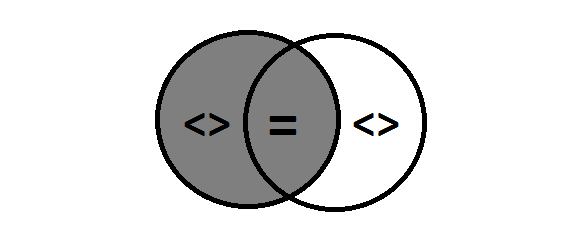
\includegraphics[width=\linewidth]{images/part_4_notes_10.png}
    \end{center}

    \bigskip

    \begin{enumerate}[A.]
        \item INNER JOIN
        \item FULL JOIN
        \item RIGHT OUTER JOIN
        \item LEFT OUTER JOIN
    \end{enumerate}

    \bigskip

    \textbf{Answer:} D

\end{enumerate}


\bigskip

\section{Review and Practice}

\bigskip

\section{Exercise 1}

\bigskip

\begin{itemize}
    \item Solution included in \textit{exercise\_1.sql}
\end{itemize}


\end{document}